The vertices of rectangle OKAY are
\begin{align}
\vec{O}&= \myvec{0\\0},\vec{K}= \myvec{a\\0},\vec{A}= \myvec{0\\c},\vec{Y}= \myvec{a\\c}
\implies \vec{O}= \myvec{0\\0},\vec{K}= \myvec{7\\0},\vec{A}= \myvec{0\\5},\vec{Y}= \myvec{7\\5}
\end{align}
See Fig.   \ref{sep/2/12/fig:RECTANGLE OKAY}
\begin{figure}[h!]
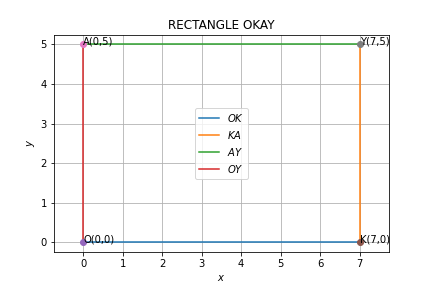
\includegraphics[width=\columnwidth]{solutions/sep/2/12/RECTANGLE.png}
  \caption{RECTANGLE OKAY }
  \label{sep/2/12/fig:RECTANGLE OKAY}
\end{figure}
